\documentclass[journal,onecolumn]{IEEEtran}

\usepackage{graphicx}
\usepackage{amsmath}
\usepackage{amssymb}
\usepackage{booktabs}
\usepackage{hyperref}
\usepackage{float}
\usepackage{subcaption}
\usepackage[margin=1in]{geometry}
\usepackage{cite}

\title{E0 270(0): Assignment 1 \\ Gaussian Naive Bayes \& Active Learning}
\author{Shashank Sekhar\\SR No.\ 26156}
\date{}

\begin{document}

\maketitle

\begin{abstract}
This report covers my GNB implementation for the breast cancer dataset and the active learning experiments I ran on top of it. The best configuration I found ended up being Yeo-Johnson with $\epsilon=10^{-3}$ smoothing, which gave 98.57\% on the test set. For active learning, uncertainty sampling got to the full-data baseline using around 17\% of the labels.
\end{abstract}

% ============================================================
\section{Problem 1: Gaussian Naive Bayes Classification}
% ============================================================

\subsection{Data and Preprocessing}

The data consists of \texttt{train1.csv} (499 samples, 30 features each) and \texttt{test1.csv} (70 samples). These are FNA image measurements from breast masses, and the label is either M (malignant) or B (benign). I encoded M as 1 and B as 0.

I split \texttt{train1.csv} into 348 training and 151 validation samples using a stratified 70/30 split, seeded with \texttt{sr\_no = 26156} so it's reproducible. For missing values, I computed column-wise medians on the training portion and used those same medians to fill in the validation and test sets too (to avoid any data leakage).

\subsection{GNB Assumption Analysis}

Before jumping into training, I wanted to check how well the data actually fits what GNB assumes.

\begin{figure}[H]
    \centering
    \begin{subfigure}[b]{0.48\textwidth}
        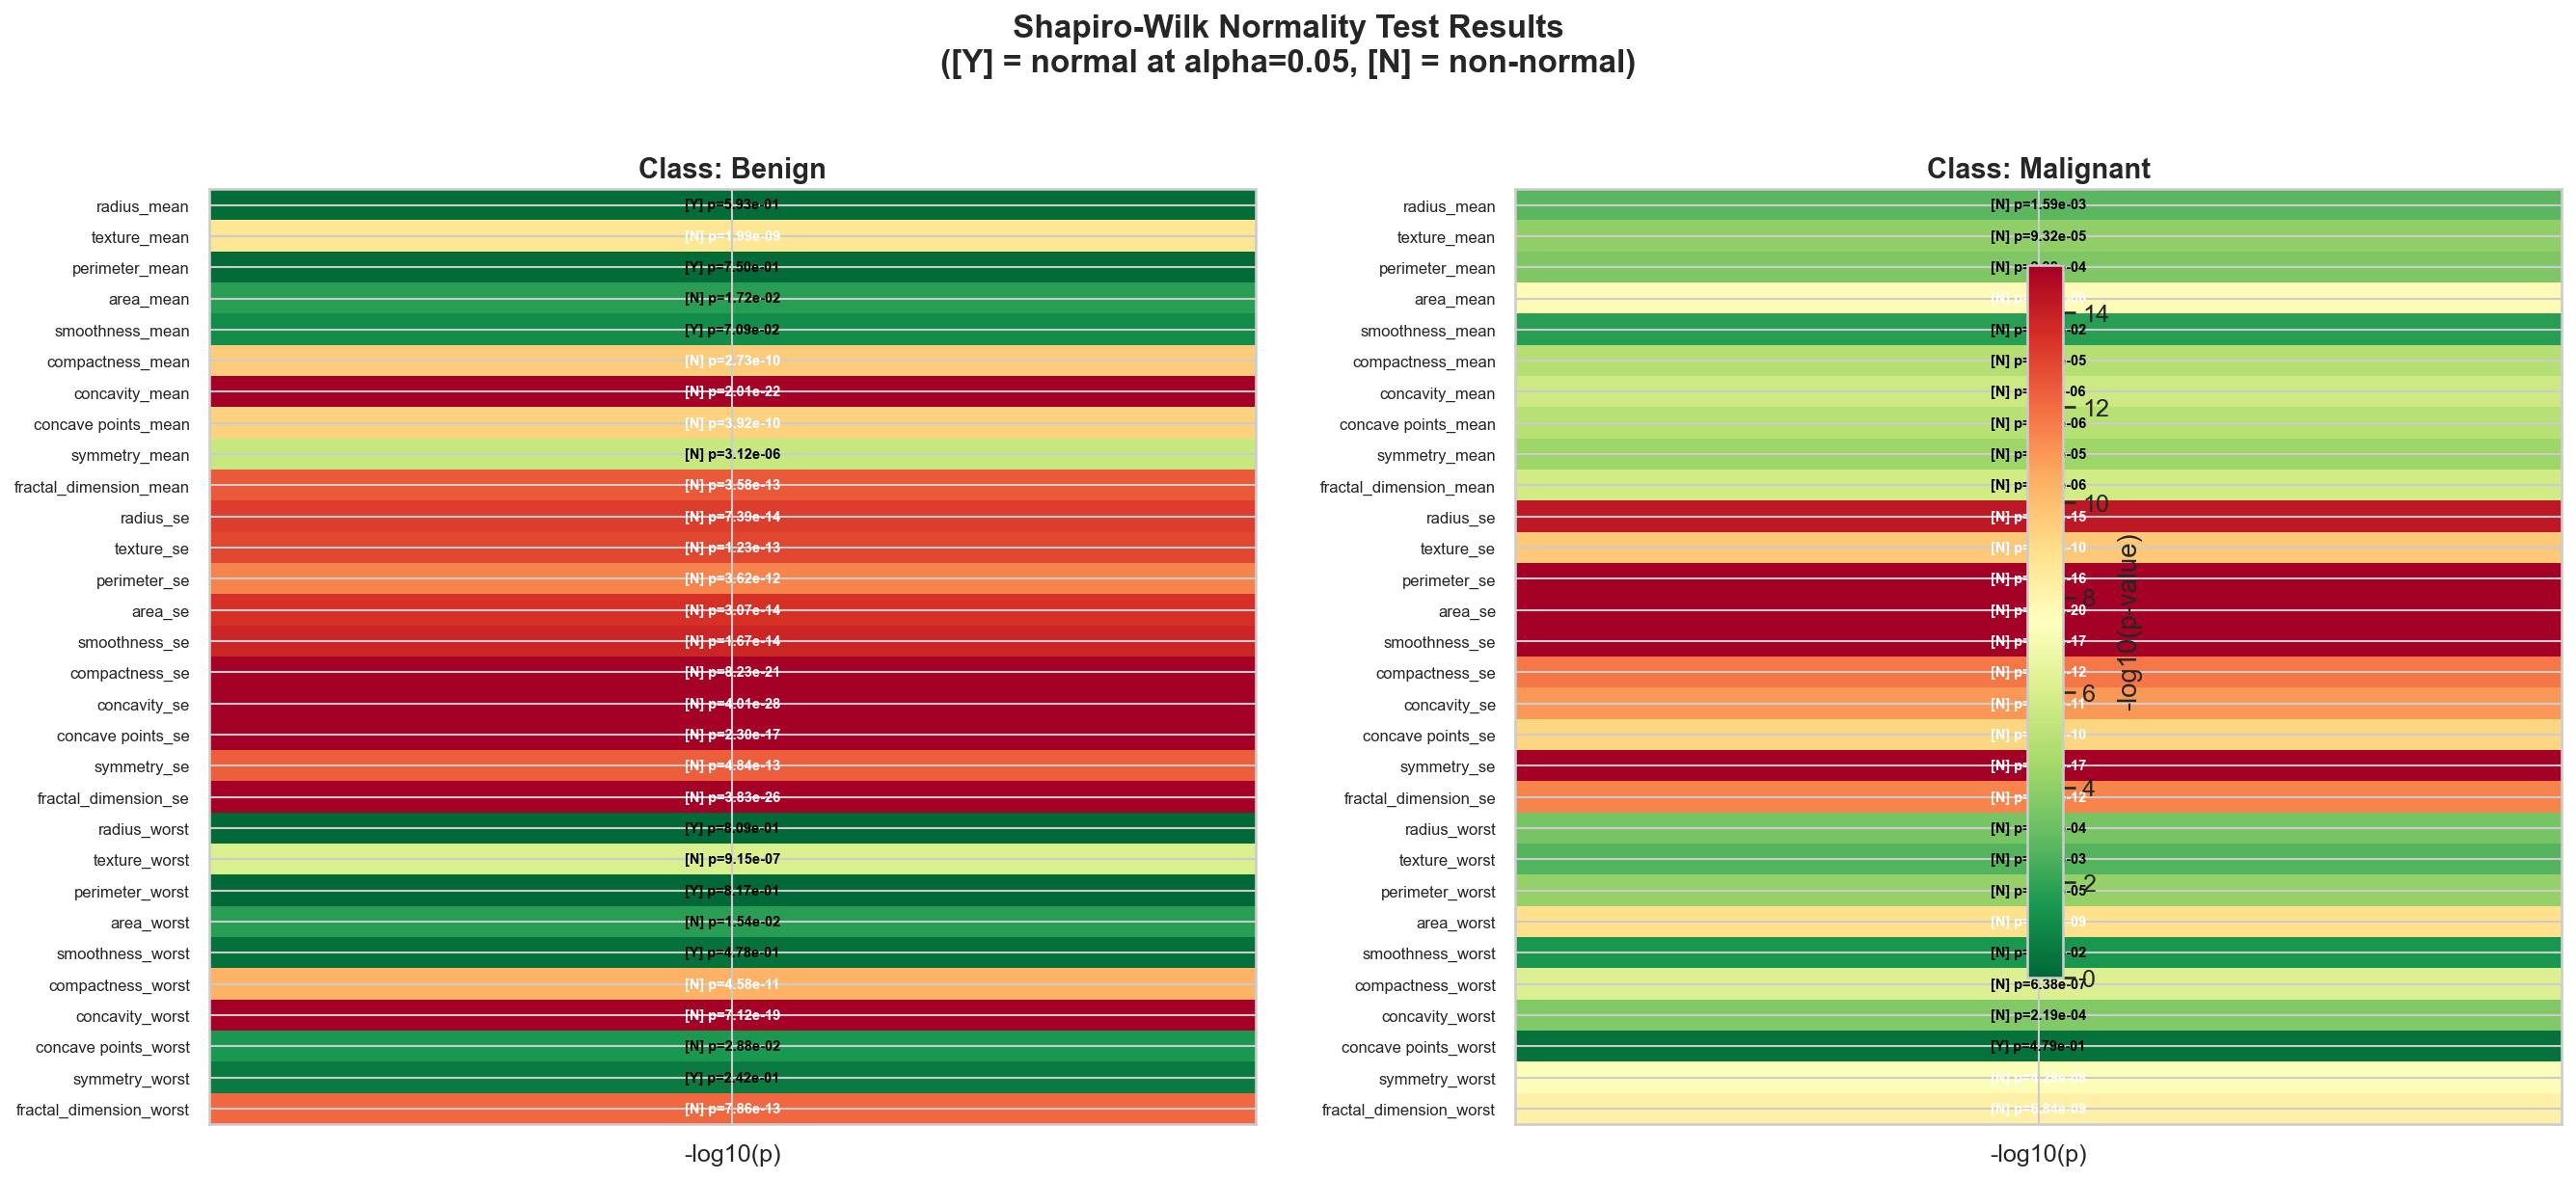
\includegraphics[width=\textwidth]{plots/assumption_analysis/1a_normality_heatmap.png}
        \caption{Shapiro-Wilk normality test results per feature and class. Green = normal ($p > 0.05$), red = non-normal.}
        \label{fig:normality_heatmap}
    \end{subfigure}
    \hfill
    \begin{subfigure}[b]{0.48\textwidth}
        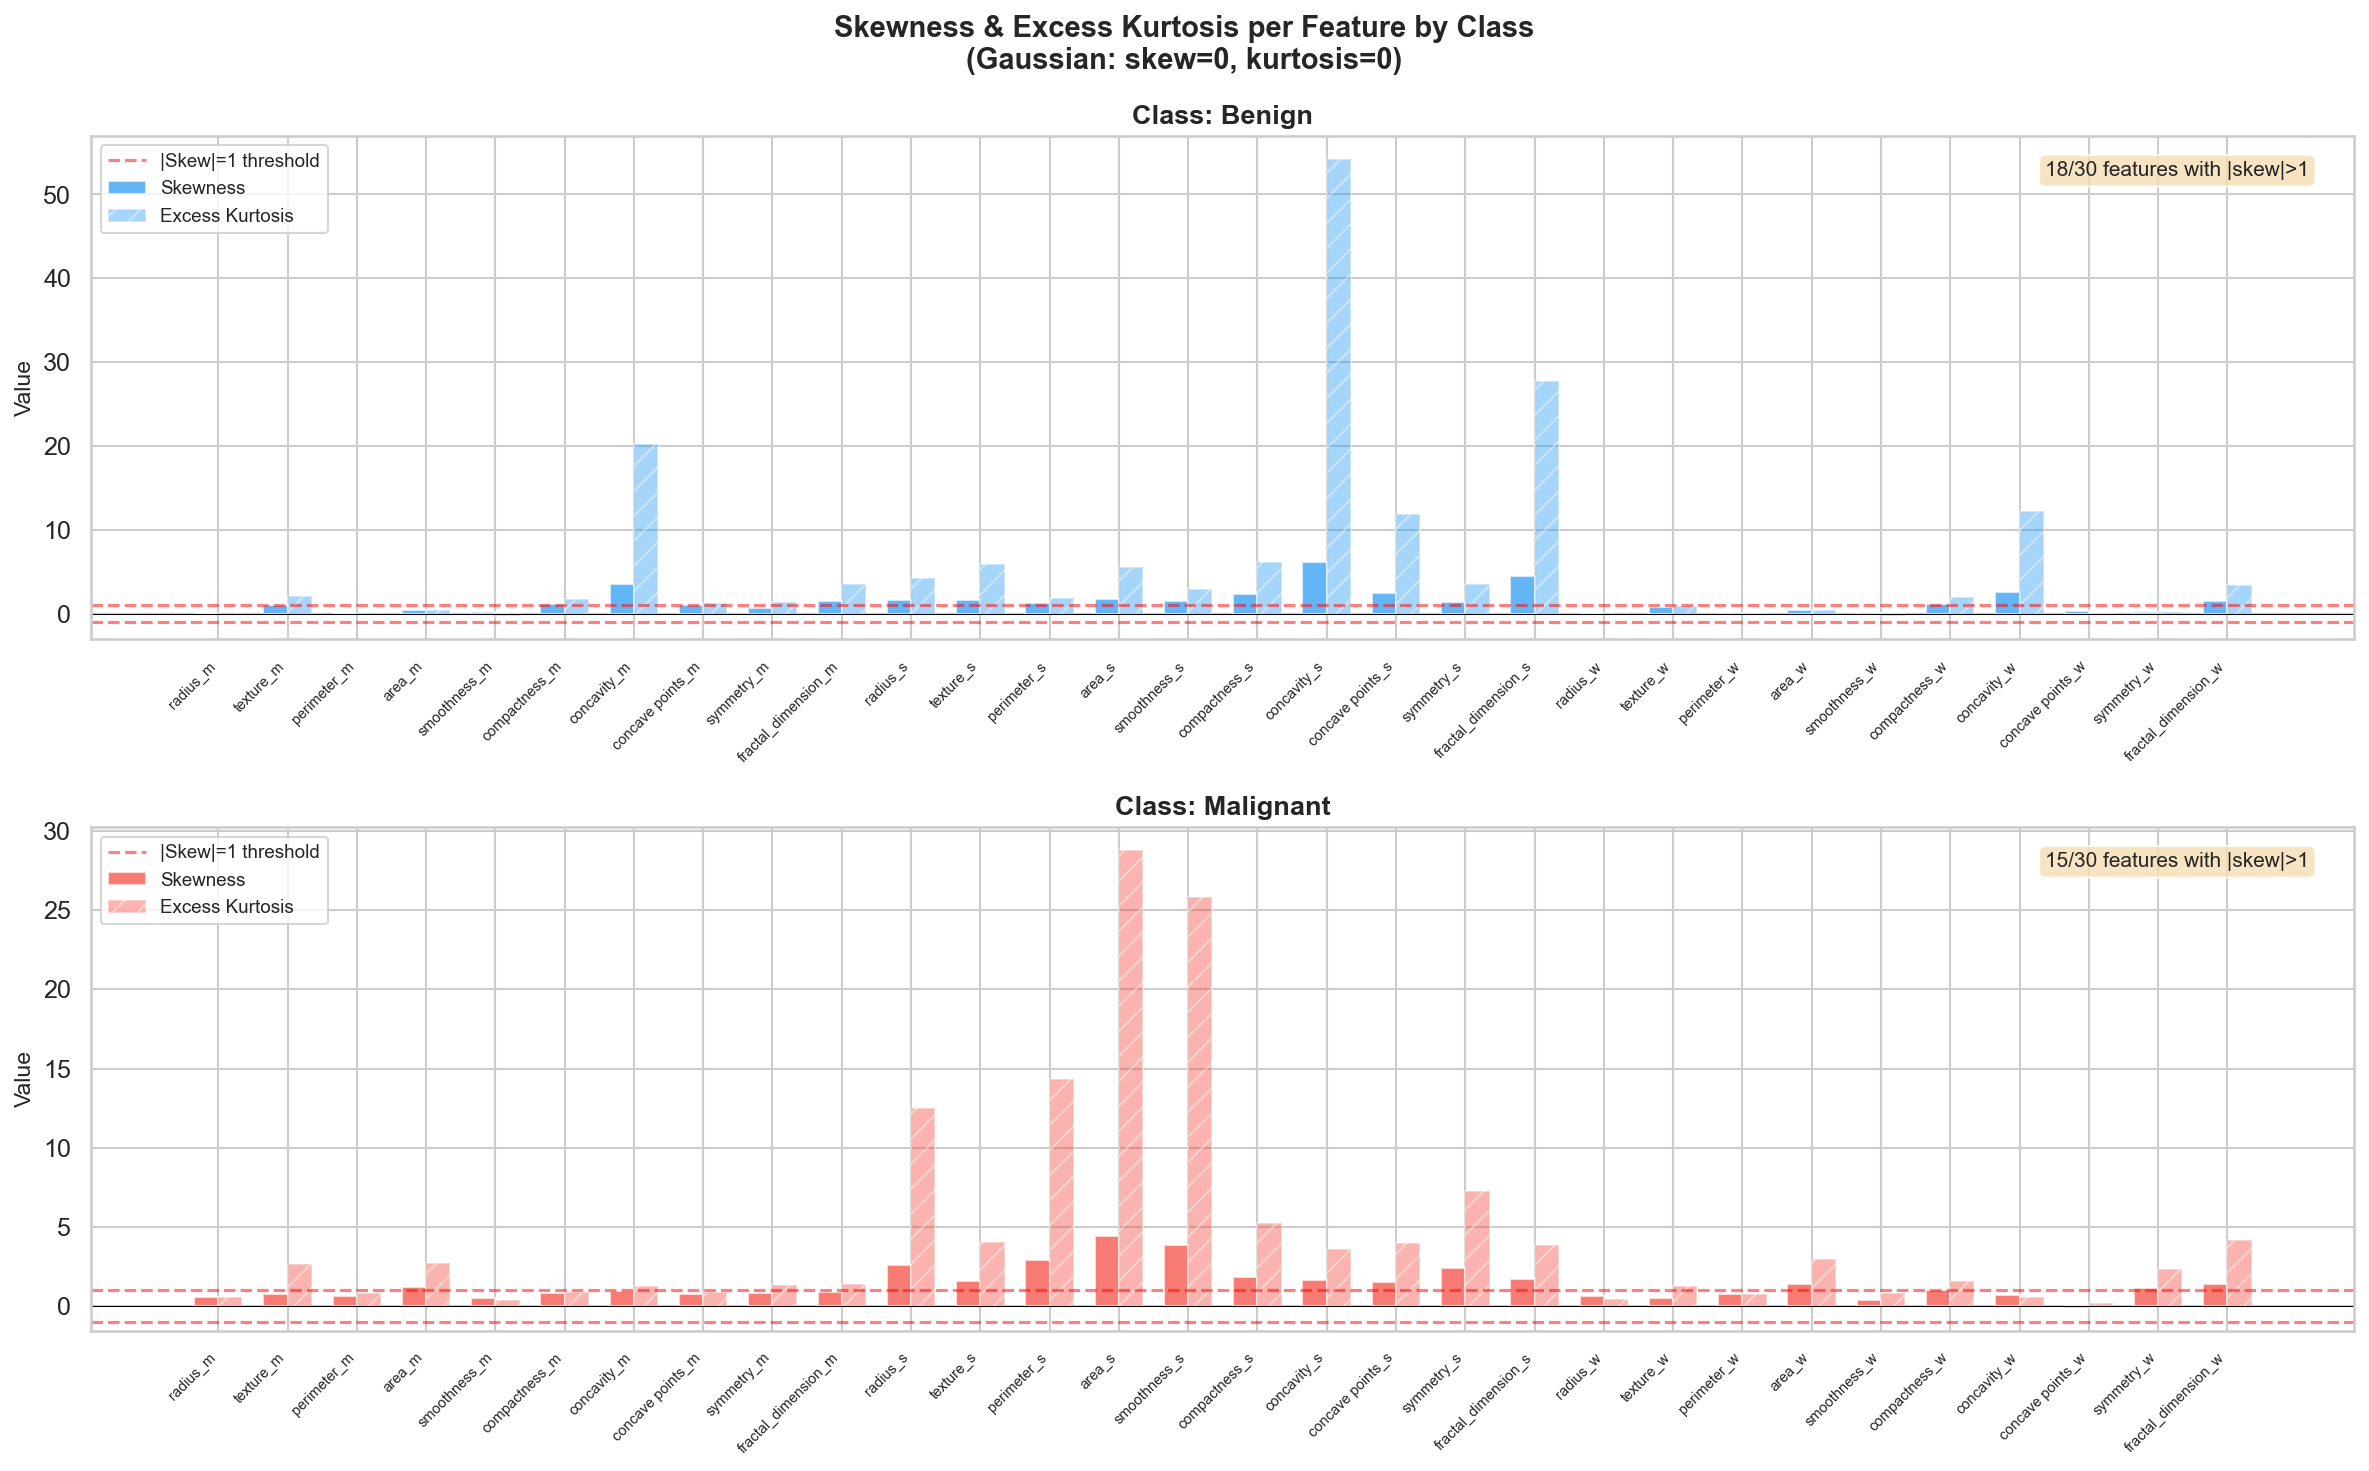
\includegraphics[width=\textwidth]{plots/assumption_analysis/3_skewness_kurtosis.png}
        \caption{Skewness and kurtosis of each feature by class. Many features exhibit high skewness, violating normality.}
        \label{fig:skewness}
    \end{subfigure}
    \caption{Normality analysis of the training data.}
    \label{fig:normality_analysis}
\end{figure}

\begin{table}[H]
\centering
\caption{GNB Assumption Summary}
\label{tab:assumption_summary}
\begin{tabular}{lccccc}
\toprule
\textbf{Class} & \textbf{N} & \textbf{Normal Features} & \textbf{Pairs $|r|>0.9$} & \textbf{Mean $|r|$} & \textbf{Highly Skewed} \\
\midrule
B (Benign) & 305 & 7/30 (23\%) & 18 & 0.309 & 18/30 (60\%) \\
M (Malignant) & 194 & 1/30 (3\%) & 17 & 0.337 & 15/30 (50\%) \\
\bottomrule
\end{tabular}
\end{table}

Looking at Table~\ref{tab:assumption_summary}, it's pretty clear the Gaussian assumption doesn't hold well only 23\% of features pass the Shapiro-Wilk test for benign and just 3\% for malignant. More than half are heavily skewed ($|s|>1$) too. This is what made me try power transforms later on. I also noticed 17--18 feature pairs with $|r|>0.9$, so I tried dropping some of them, but that actually made accuracy worse (more on this in Section~\ref{sec:feature_eng}).

\begin{figure}[H]
    \centering
    \begin{subfigure}[b]{0.48\textwidth}
        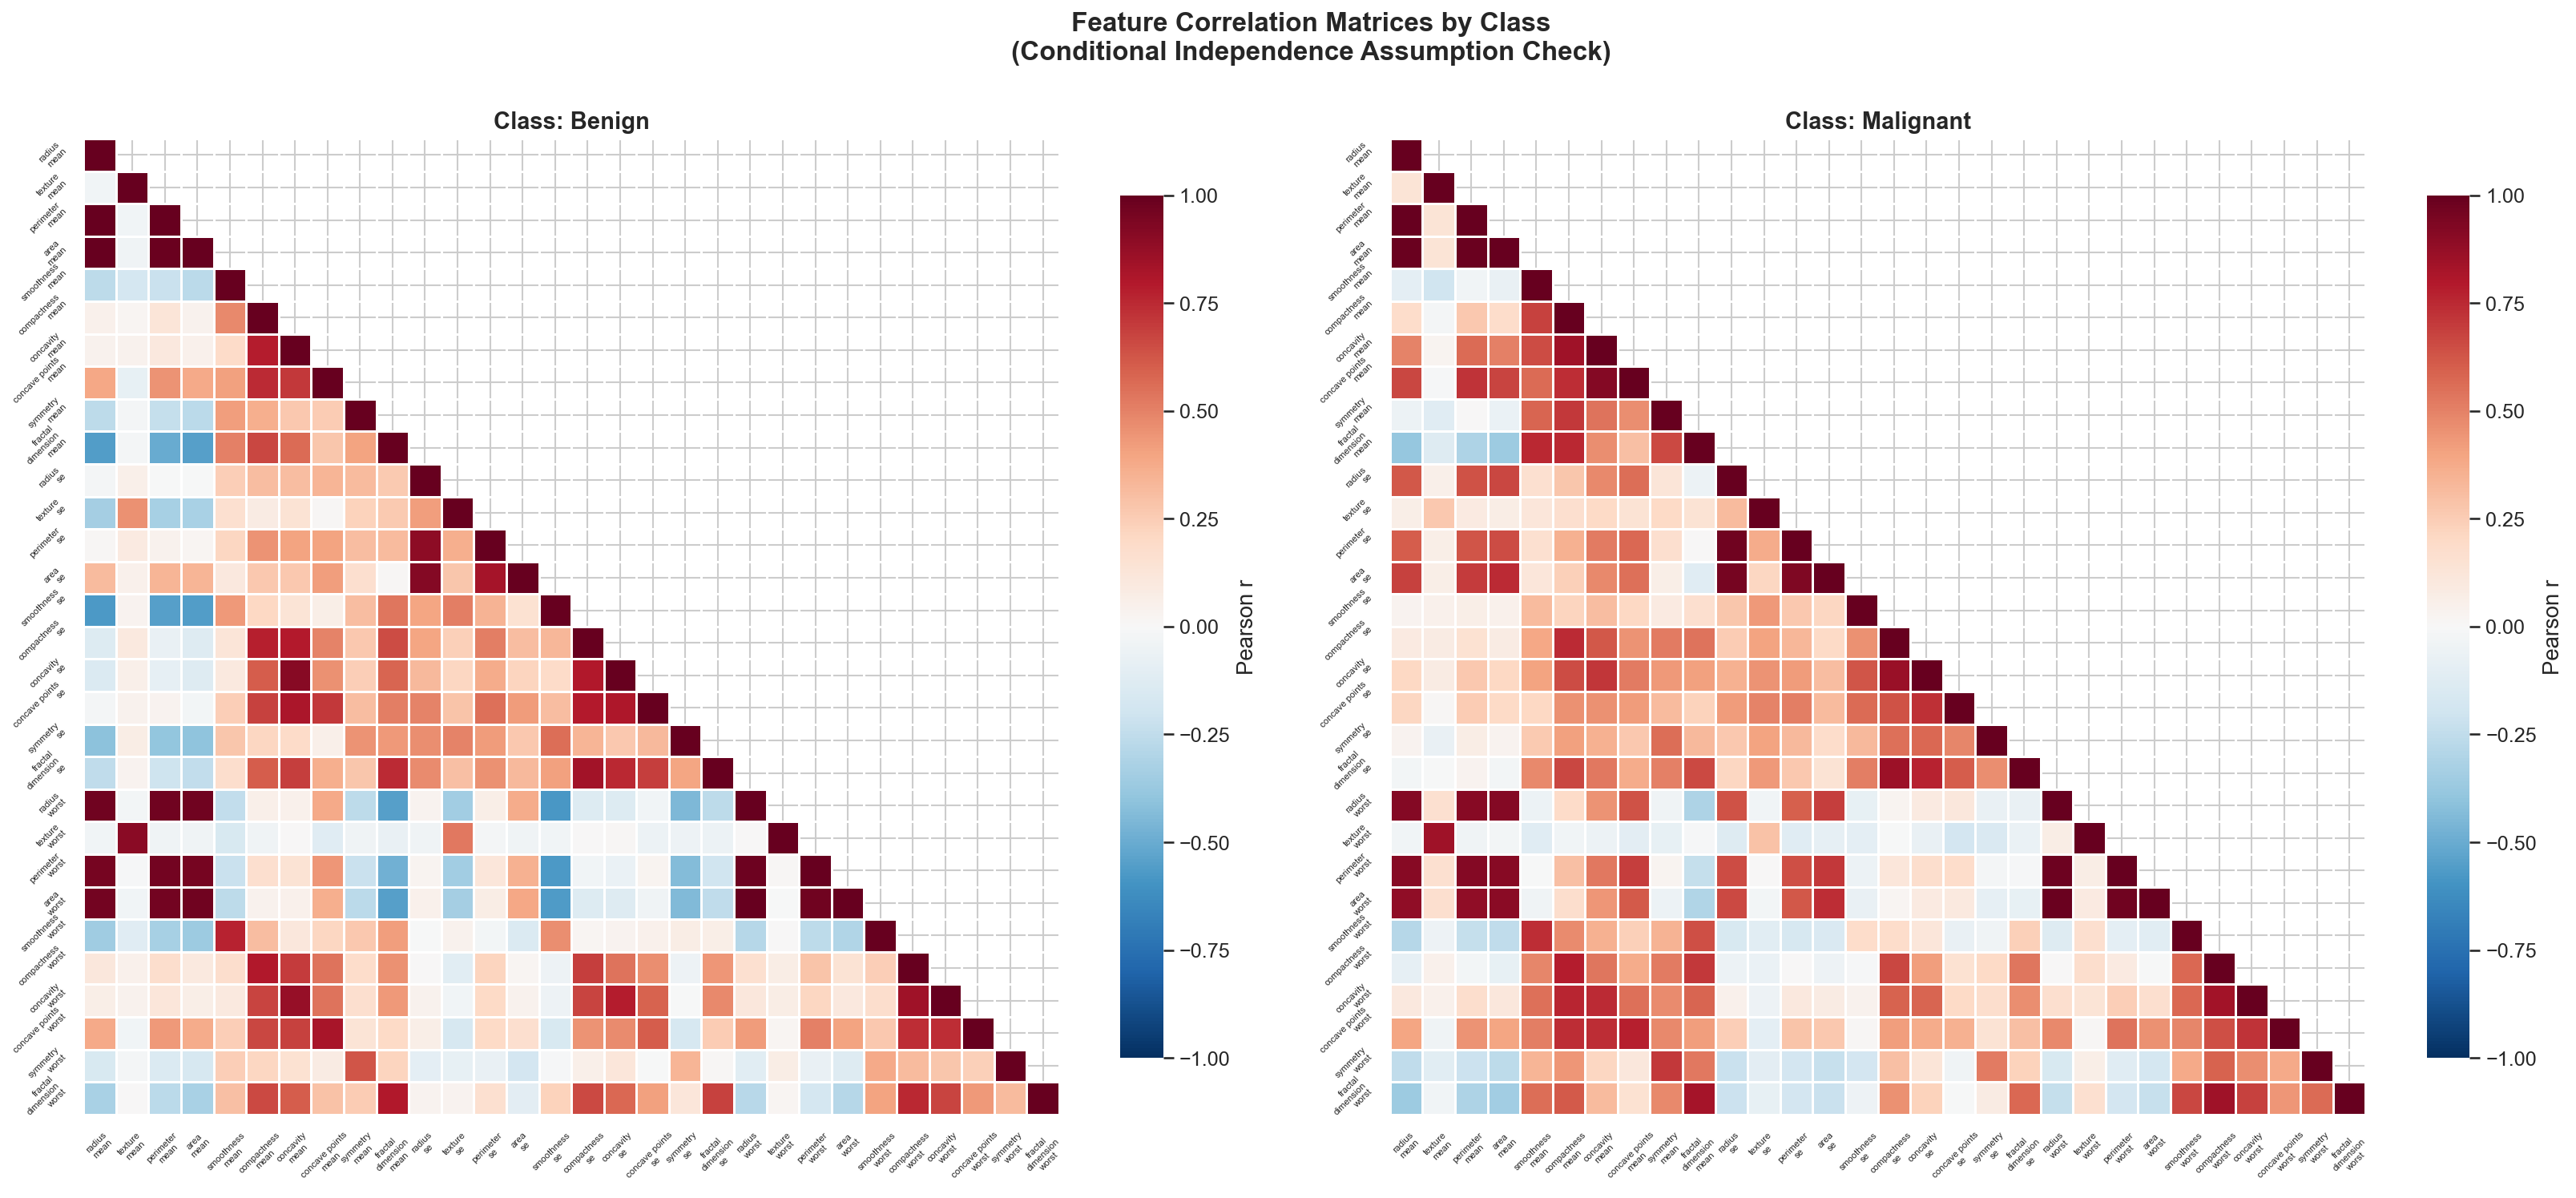
\includegraphics[width=\textwidth]{plots/assumption_analysis/2a_correlation_heatmaps.png}
        \caption{Feature correlation heatmaps by class.}
        \label{fig:corr_heatmap}
    \end{subfigure}
    \hfill
    \begin{subfigure}[b]{0.48\textwidth}
        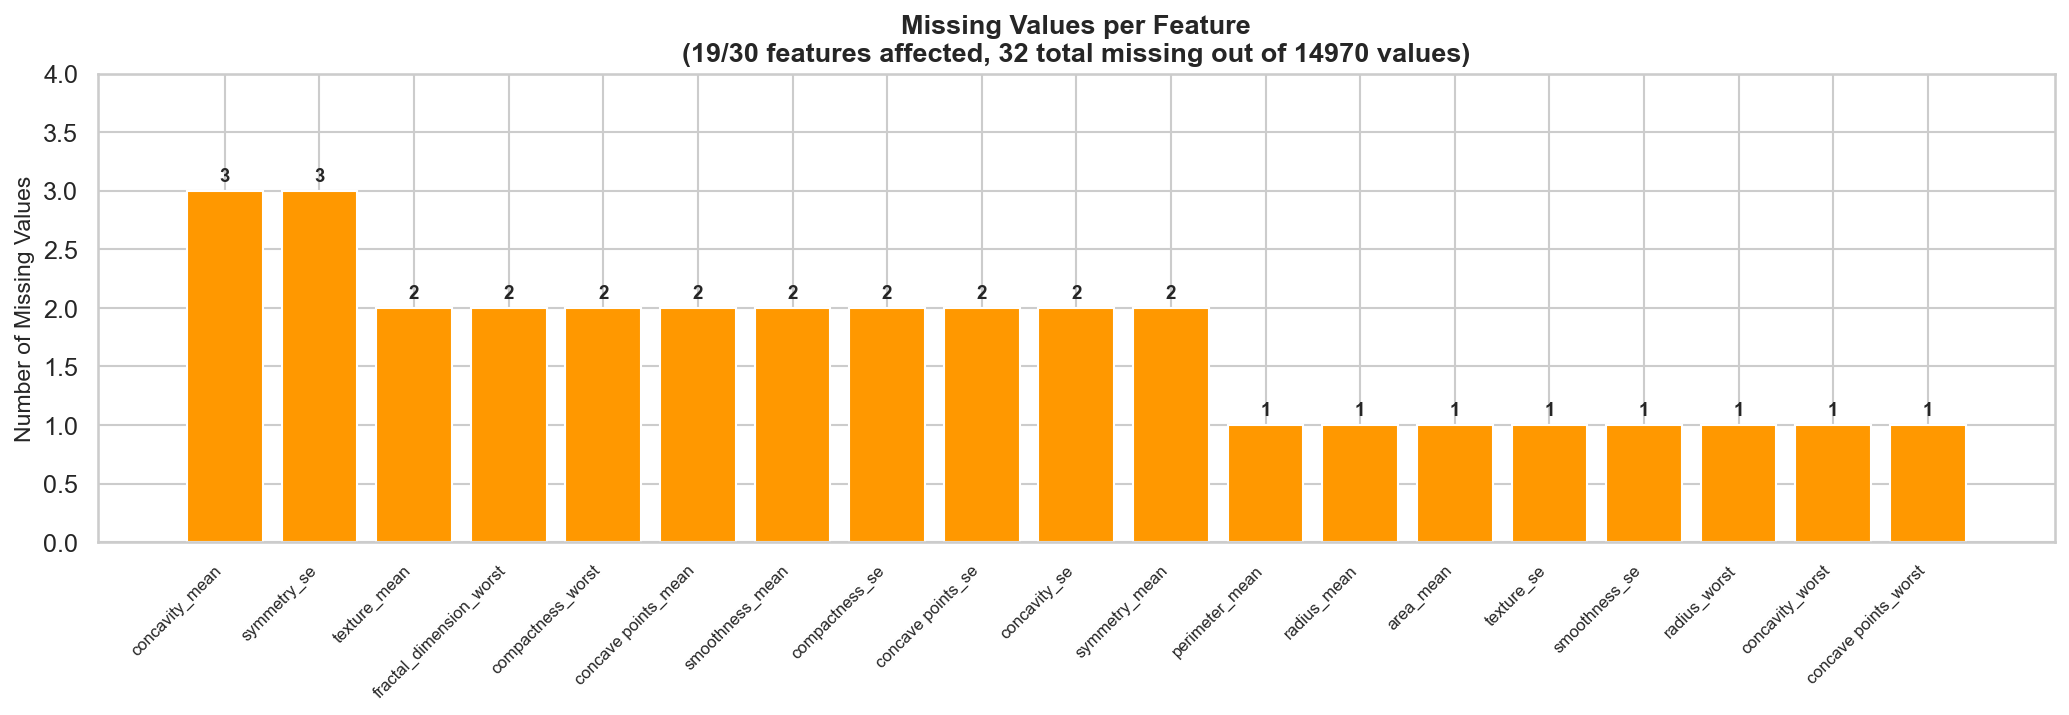
\includegraphics[width=\textwidth]{plots/assumption_analysis/4_missing_data.png}
        \caption{Missing data pattern across features.}
        \label{fig:missing_data}
    \end{subfigure}
    \caption{Correlation structure and missing data analysis.}
    \label{fig:corr_missing}
\end{figure}

\subsection{Model Implementation}

The standard GNB posterior for class $c$ given input $\mathbf{x} = (x_1, \ldots, x_d)$ is:

\begin{equation}
    P(c \mid \mathbf{x}) = \frac{P(c) \prod_{j=1}^{d} P(x_j \mid c)}{\sum_{c'} P(c') \prod_{j=1}^{d} P(x_j \mid c')}
\end{equation}

I model each $P(x_j \mid c)$ as a Gaussian:
\begin{equation}
    P(x_j \mid c) = \frac{1}{\sqrt{2\pi(\sigma_{cj}^2 + \epsilon)}} \exp\left(-\frac{(x_j - \mu_{cj})^2}{2(\sigma_{cj}^2 + \epsilon)}\right)
\end{equation}
Here $\mu_{cj}$, $\sigma_{cj}^2$ are the per-class mean and variance for feature $j$, and $\epsilon$ is a smoothing term I add to all variances so nothing blows up.

In my implementation, all the computation happens in log-space because the raw products would underflow to zero otherwise. So the log-posterior ends up being:
\begin{equation}
    \log P(c \mid \mathbf{x}) \propto \log P(c) + \sum_{j=1}^{d} \left[ -\frac{1}{2}\log(2\pi\hat{\sigma}_{cj}^2) - \frac{(x_j - \mu_{cj})^2}{2\hat{\sigma}_{cj}^2} \right]
\end{equation}
with $\hat{\sigma}_{cj}^2 = \sigma_{cj}^2 + \epsilon$. When I need actual probabilities (for \texttt{predict\_proba}), I normalize using the log-sum-exp trick:
\begin{equation}
    P(c \mid \mathbf{x}) = \frac{\exp(\log P_c^* - M)}{\sum_{c'}\exp(\log P_{c'}^* - M)}, \quad M = \max_{c'} \log P_{c'}^*
\end{equation}

I tried both empirical priors ($P(c) = N_c / N$) and uniform ones ($P(c) = 1/K$) to see which works better.

\subsection{Feature Engineering}
\label{sec:feature_eng}

Based on the assumption analysis, I figured applying some kind of power transform might help since so many features are skewed. I went with Yeo-Johnson~\cite{yeo2000} instead of Box-Cox because Box-Cox can't handle zero or negative values. Apart from that, I also experimented with winsorization (clipping outliers at the 5th/95th percentile) and dropping highly correlated features. In total I had seven variants:

\begin{enumerate}
    \item[\textbf{A.}] \textbf{Vanilla Implementation}
    \item[\textbf{B.}] \textbf{Power transform}: Yeo-Johnson transform applied to each feature to reduce skewness and improve normality. Parameters are fit on the training set only.
    \item[\textbf{C.}] \textbf{Remove correlated}: Features with pairwise $|r| > 0.9$ are removed (keeping one from each pair).
    \item[\textbf{D.}] \textbf{Power + Remove correlated}: Combination of B and C.
    \item[\textbf{E.}] \textbf{Winsorize}: Outliers are clipped to the 5th/95th percentile bounds (computed on training set).
    \item[\textbf{F.}] \textbf{Winsorize + Power}: Combination of E and B.
    \item[\textbf{G.}] \textbf{Winsorize + Power + Remove correlated}: Combination of E, B, and C.
\end{enumerate}

\subsection{Hyperparameter Tuning}

I ran a grid search over all 7 variants, 4 smoothing values ($10^{-9}$, $10^{-6}$, $10^{-3}$, $10^{-1}$), and both prior types---so 56 configurations total. Table~\ref{tab:top10_configs} shows the top 10.

\begin{table}[H]
\centering
\caption{Top 10 Configurations by Validation Accuracy}
\label{tab:top10_configs}
\begin{tabular}{llccccc}
\toprule
\textbf{Variant} & \textbf{Prior} & $\boldsymbol{\epsilon}$ & \textbf{Val Acc} & \textbf{F1 (macro)} & \textbf{ROC-AUC} & \textbf{Recall (macro)} \\
\midrule
B\_power\_transform & empirical & $10^{-3}$ & \textbf{0.9669} & 0.9655 & 0.9959 & 0.9698 \\
B\_power\_transform & uniform & $10^{-3}$ & 0.9669 & 0.9657 & 0.9959 & 0.9728 \\
F\_winsor+power & empirical & $10^{-3}$ & 0.9603 & 0.9585 & 0.9954 & 0.9613 \\
B\_power\_transform & uniform & $10^{-9}$ & 0.9536 & 0.9520 & 0.9959 & 0.9589 \\
B\_power\_transform & empirical & $10^{-9}$ & 0.9536 & 0.9520 & 0.9961 & 0.9589 \\
F\_winsor+power & uniform & $10^{-9}$ & 0.9536 & 0.9520 & 0.9961 & 0.9589 \\
F\_winsor+power & empirical & $10^{-9}$ & 0.9536 & 0.9520 & 0.9961 & 0.9589 \\
F\_winsor+power & uniform & $10^{-3}$ & 0.9536 & 0.9517 & 0.9954 & 0.9559 \\
A\_vanilla & uniform & $10^{-3}$ & 0.9404 & 0.9379 & 0.9913 & 0.9335 \\
E\_winsorize & uniform & $10^{-3}$ & 0.9404 & 0.9379 & 0.9912 & 0.9335 \\
\bottomrule
\end{tabular}
\end{table}

The power transform configs took all the top spots, and $\epsilon = 10^{-3}$ was consistently the best smoothing value. What I didn't expect was that removing correlated features (variants C, D, G) always made things worse---I thought it would help given the high correlations, but apparently GNB still gets something useful out of those ``redundant'' features. Adding winsorization on top of power transform (F) wasn't really worth it either.

\subsection{Test Set Evaluation}

I then took the best config (B\_power\_transform, $\epsilon = 10^{-3}$, empirical priors) and ran it on \texttt{test1.csv}. Table~\ref{tab:test_results} has the full results.

\begin{table}[H]
\centering
\caption{Test Set Results (Best Configuration)}
\label{tab:test_results}
\begin{tabular}{lcc}
\toprule
\textbf{Metric} & \textbf{Default Threshold (0.5)} & \textbf{Tuned Threshold (0.8728)} \\
\midrule
Accuracy & \textbf{0.9857} & 0.9714 \\
Precision (macro) & 0.9737 & 0.9626 \\
Recall (macro) & 0.9904 & 0.9626 \\
F1 (macro) & 0.9816 & 0.9626 \\
F1 (weighted) & 0.9858 & --- \\
ROC-AUC & 0.9979 & --- \\
False Negatives & \textbf{0} & 1 \\
False Positives & 1 & 1 \\
\bottomrule
\end{tabular}
\end{table}

At the default 0.5 threshold it gets 98.57\% accuracy and doesn't miss any cancer cases (zero false negatives), which is good because in this kind of application you really don't want to miss a malignant one. ROC-AUC came out to 0.9979.

I also tried tuning the threshold---I looked for the highest value that still keeps recall $\geq 0.95$ on the validation set, and that ended up being 0.8728. With that threshold, test accuracy drops a bit to 97.14\%. Since the default threshold was already getting perfect recall on malignant cases anyway, the tuning didn't really change much in this case.

\begin{figure}[H]
    \centering
    \begin{subfigure}[b]{0.48\textwidth}
        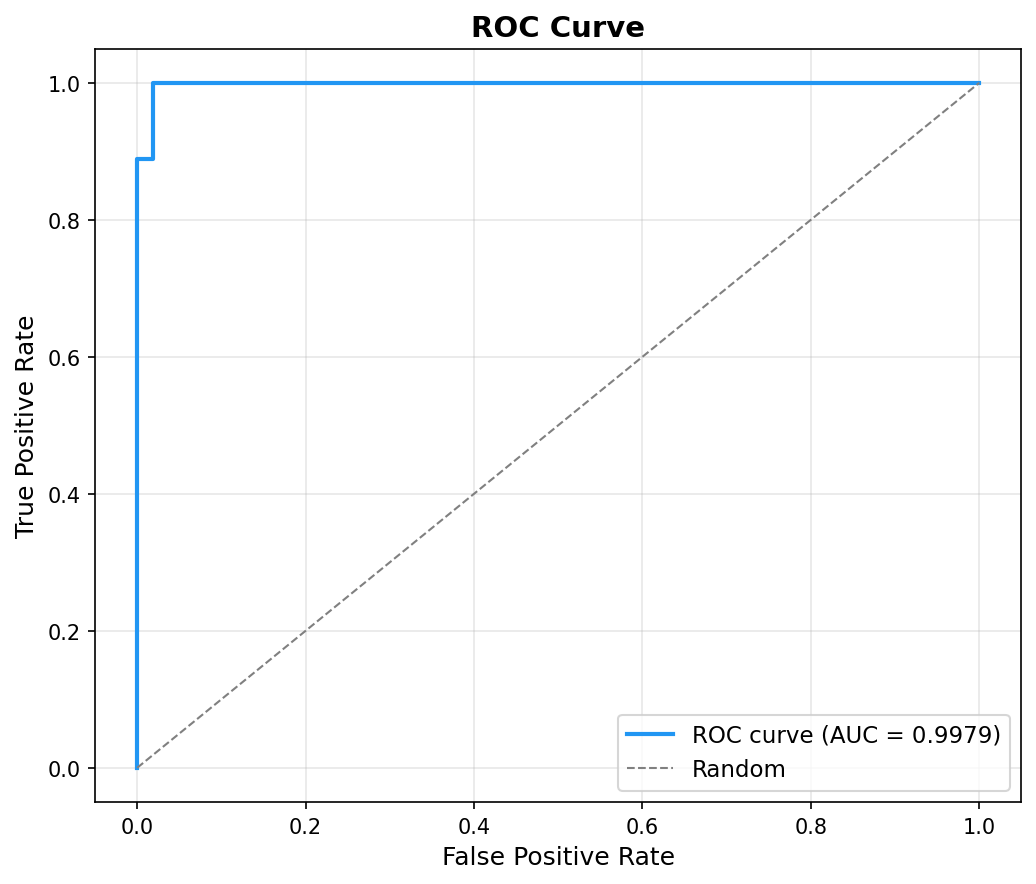
\includegraphics[width=\textwidth]{plots/prob1/roc_curve.png}
        \caption{ROC curve (AUC = 0.9979).}
        \label{fig:roc}
    \end{subfigure}
    \hfill
    \begin{subfigure}[b]{0.48\textwidth}
        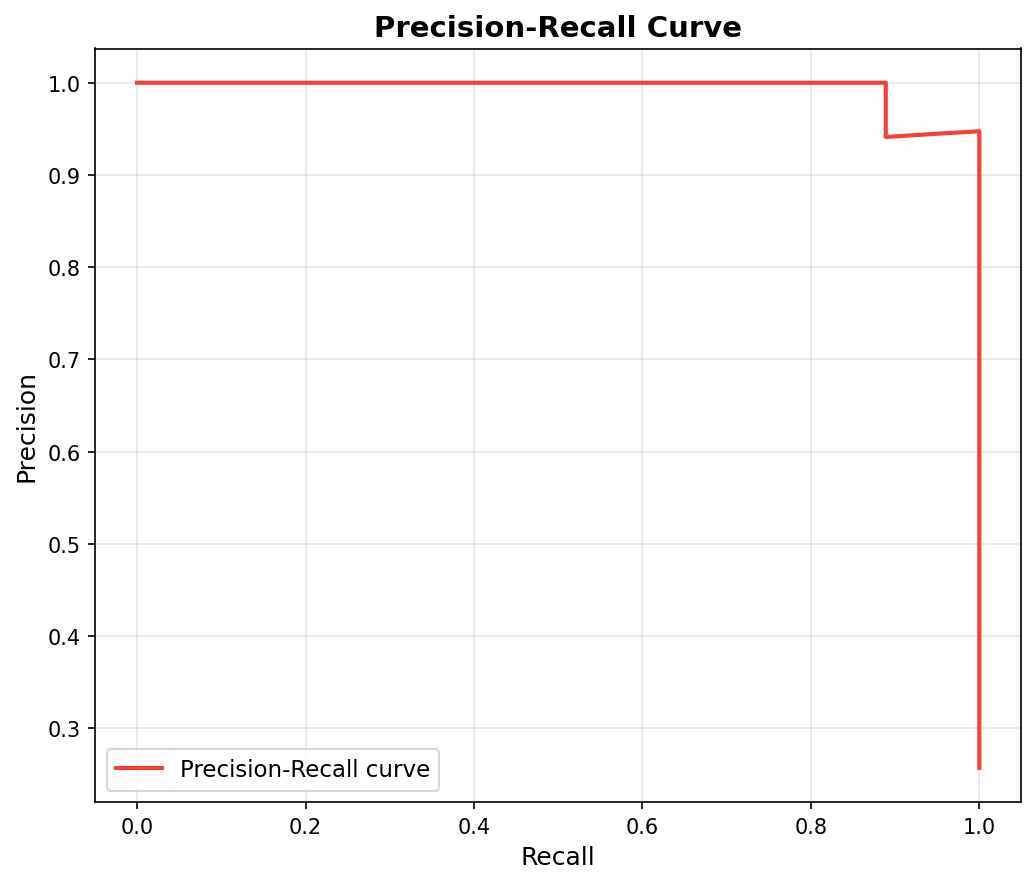
\includegraphics[width=\textwidth]{plots/prob1/pr_curve.png}
        \caption{Precision-Recall curve.}
        \label{fig:pr}
    \end{subfigure}
    \caption{ROC and Precision-Recall curves on the test set.}
    \label{fig:roc_pr}
\end{figure}

\begin{figure}[H]
    \centering
    \begin{subfigure}[b]{0.48\textwidth}
        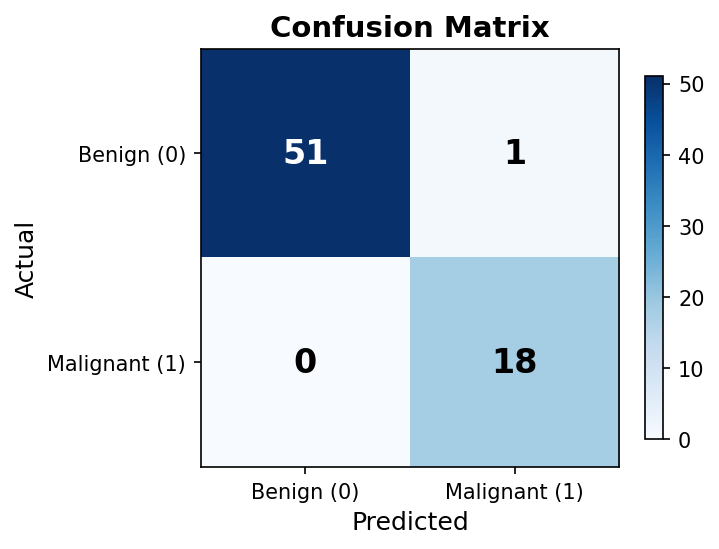
\includegraphics[width=\textwidth]{plots/prob1/confusion_matrix.png}
        \caption{Default threshold (0.5).}
        \label{fig:cm_default}
    \end{subfigure}
    \hfill
    \begin{subfigure}[b]{0.48\textwidth}
        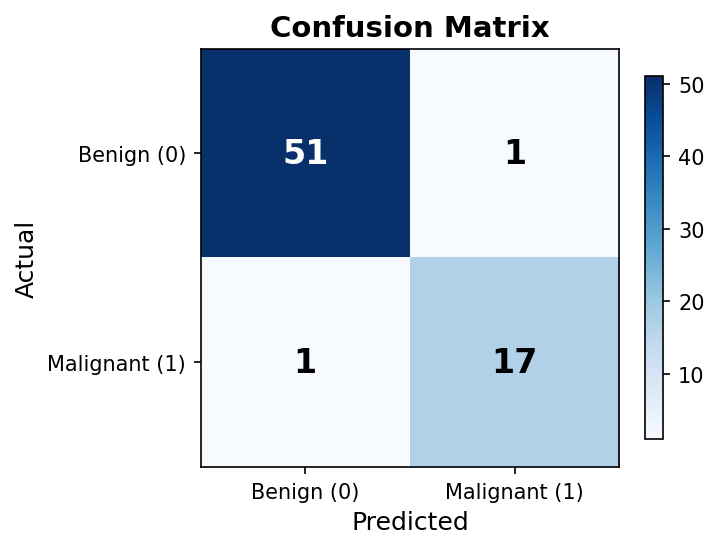
\includegraphics[width=\textwidth]{plots/prob1/confusion_matrix_tuned.png}
        \caption{Tuned threshold (0.8728) for recall $\geq$ 0.95.}
        \label{fig:cm_tuned}
    \end{subfigure}
    \caption{Confusion matrices on the test set.}
    \label{fig:confusion}
\end{figure}

% ============================================================
\section{Problem 2: Active Learning with Incremental GNB}
% ============================================================

\subsection{Active Learning Strategy}

For this part, instead of randomly picking which samples to label next, I let the model decide. The strategy I used is uncertainty sampling~\cite{settles2012} basically, look at all the unlabeled samples, see which ones the model is most confused about (predicted probability near 0.5), and label those first. The thinking is that those borderline samples give the model more information than easy ones it's already confident about.

Here's how I set up the loop: I start with 20 randomly chosen labeled samples (seed is \texttt{sr\_no + run\_id} so each run is different but reproducible). Then each iteration I add 10 more. For the active strategy (ALS), I pick the 10 unlabeled samples whose $P(\text{malignant} \mid \mathbf{x})$ is closest to 0.5. For the passive/random baseline, I just take the next 10 from a pre-shuffled list. After adding each batch I evaluate on the validation set, and I keep going until there's nothing left to label or I hit 39 iterations.

\subsection{Incremental Model Update via Sufficient Statistics}

One nice thing about GNB is that I don't have to retrain on all the data every time I add a new batch. Since the model only stores per-class counts $n_c$, means $\boldsymbol{\mu}_c$, and variances $\boldsymbol{\sigma}_c^2$, I can just merge the old statistics with the new batch's statistics directly.

If I have old stats $(n_c^{\text{old}}, \boldsymbol{\mu}_c^{\text{old}}, (\boldsymbol{\sigma}_c^{\text{old}})^2)$ and the new batch gives $(n_c^{\text{new}}, \boldsymbol{\mu}_c^{\text{new}}, (\boldsymbol{\sigma}_c^{\text{new}})^2)$, the update formulas are:

\begin{align}
    n_c &= n_c^{\text{old}} + n_c^{\text{new}} \\
    \boldsymbol{\mu}_c &= \frac{n_c^{\text{old}} \boldsymbol{\mu}_c^{\text{old}} + n_c^{\text{new}} \boldsymbol{\mu}_c^{\text{new}}}{n_c} \\
    \boldsymbol{\sigma}_c^2 &= \frac{n_c^{\text{old}}((\boldsymbol{\sigma}_c^{\text{old}})^2 + (\boldsymbol{\mu}_c^{\text{old}})^2) + n_c^{\text{new}}((\boldsymbol{\sigma}_c^{\text{new}})^2 + (\boldsymbol{\mu}_c^{\text{new}})^2)}{n_c} - \boldsymbol{\mu}_c^2
\end{align}

Priors just become $P(c) = n_c / \sum_{c'} n_{c'}$. So each update is $O(b \cdot d)$ where $b$ is the batch size, rather than $O(N \cdot d)$ if I had to retrain on everything.

\subsection{Learning Curves}

I ran this 5 times for each strategy (run\_id 1 through 5, each with seed \texttt{sr\_no + run\_id}), keeping smoothing at $10^{-3}$ from Problem~1. Figure~\ref{fig:learning_curves} shows the averaged learning curves.

\begin{figure}[H]
    \centering
    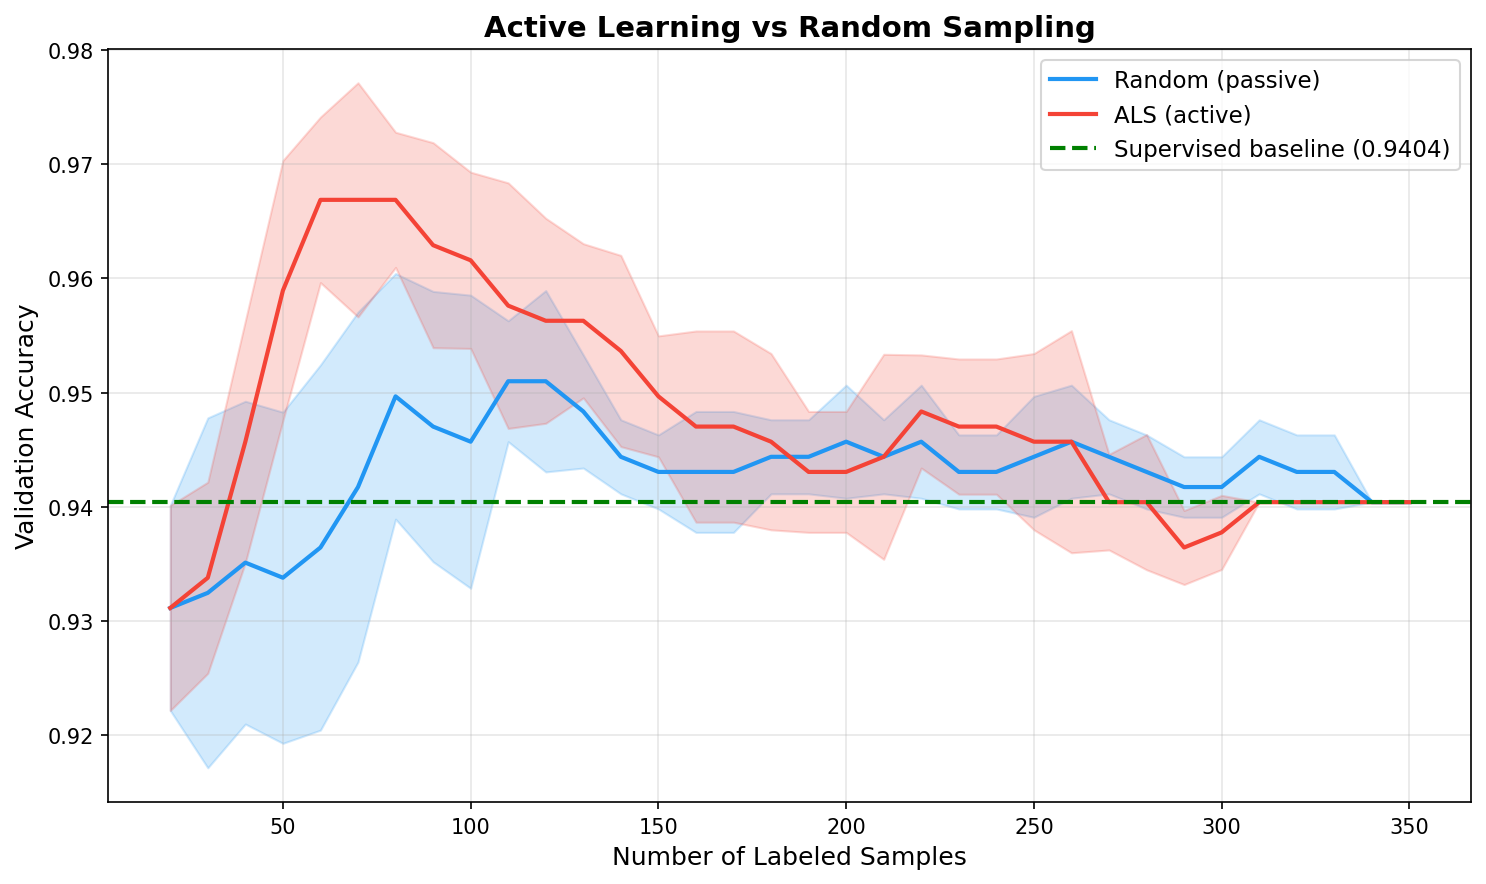
\includegraphics[width=0.75\textwidth]{plots/prob2/learning_curves.png}
    \caption{Learning curves averaged over 5 runs ($\pm 1$ std). The green dashed line is the supervised baseline (94.04\%)---what you get if you train on all 348 samples.}
    \label{fig:learning_curves}
\end{figure}

The active learning curve shoots up faster---it's already around 97\% accuracy with only 60--80 labeled samples. Random sampling takes over 100 samples to get to similar numbers. Eventually both converge to the supervised baseline once most of the data is labeled, which makes sense. Both strategies show some variance across runs; with random sampling it's because the shuffle order changes, and with ALS it's because the model's uncertainty is different depending on what it saw first.

The part I found most interesting is that ALS hits the full-data baseline at around 60 samples. That's only about 17\% of the training set, so in a real scenario where labeling is expensive, that could save a lot of effort.

\subsection{Training Time Comparison}

\begin{figure}[H]
    \centering
    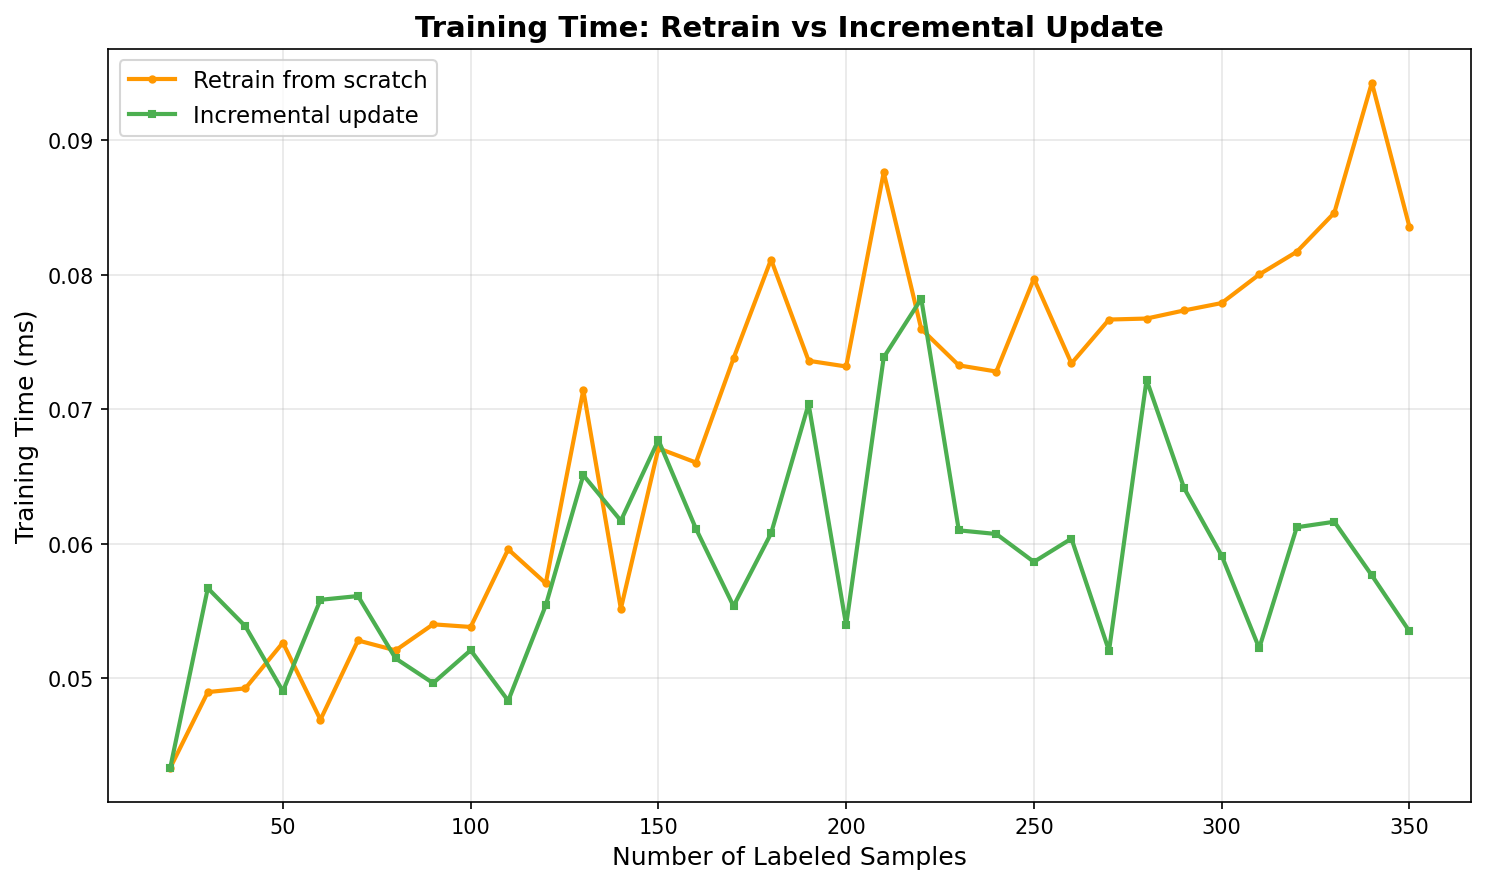
\includegraphics[width=0.75\textwidth]{plots/prob2/timing_comparison.png}
    \caption{Training time per iteration: retraining from scratch vs.\ incremental update. Times are averaged over 200 repetitions per data point to reduce noise.}
    \label{fig:timing}
\end{figure}

Figure~\ref{fig:timing} shows the timing results. The orange line (retrain from scratch) goes from about 0.04\,ms up to 0.09\,ms as the dataset grows, which makes sense since it has to process more data each time. The green line (incremental) stays flatter because it only touches the 10 new samples. It's pretty noisy since everything is under 0.1\,ms on this small dataset, but you can see the lines start to separate. I'd expect the gap to be much bigger on a larger dataset.

% ============================================================
\section{Assumptions and Justifications}
% ============================================================

A few choices I had to make along the way:

I went with median imputation over mean because a lot of the features are skewed, and the median isn't as sensitive to outliers. For the power transform I picked Yeo-Johnson over Box-Cox, Box-Cox requires strictly positive values which not all my features satisfy. I always fit the transform parameters on the training set only so there's no leakage into validation/test.

One thing that surprised me was about the correlated features. Logically, since GNB assumes independence, I expected that removing the highly correlated ones would help. But every time I tried it, accuracy went down. My best guess is that even though those features are correlated, they still carry enough useful information that GNB benefits from having them around.

For the active learning uncertainty measure I used $|P(\text{malignant}) - 0.5|$ for a binary problem this is equivalent to picking the samples with highest entropy. Initial pool size and batch size (20 and 10) are as specified in the assignment.

% ============================================================
\section{Conclusion}
% ============================================================

To sum up, my GNB classifier ended up at 98.57\% test accuracy with no missed cancer cases. The Yeo-Johnson transform made the biggest difference once I applied it, accuracy jumped noticeably compared to the vanilla model. Smoothing at $10^{-3}$ also helped. On the active learning side, uncertainty sampling reached the full-data baseline with only about 17\% of the labels, which is a pretty big saving. The incremental update worked as expected too, avoiding the need to retrain from scratch every iteration.

\begin{thebibliography}{1}

\bibitem{settles2012}
B.~Settles, ``Active learning,'' \emph{Synthesis Lectures on Artificial Intelligence and Machine Learning}, vol.~6, no.~1, pp.~1--114, 2012.

\bibitem{yeo2000}
I.-K.~Yeo and R.~A.~Johnson, ``A new family of power transformations to improve normality or symmetry,'' \emph{Biometrika}, vol.~87, no.~4, pp.~954--959, 2000.

\end{thebibliography}

\end{document}
